\section{Results}

Objective of this work is not only to device and implement a collection of algorithms for computing the midsurface,  but also to test and assess the output on real life sheet metal parts. ``Enclosure''  is a typical sheet metal casing model used in electronics equipments. It houses circuits, wires, fan, etc.

%\vspace{-0.8cm}

\def\myfigenlosurebenchmarkcolumnwidth{0.3}
\begin{figure}[!h]
\centering     %%% not \center
\subfloat[Original Part]{\label{fig:results:originalenclosurepart}\includegraphics[width=\myfigenlosurebenchmarkcolumnwidth\linewidth,valign=t]{../Common/images/SheetMetal_Medium_Enclosure_OriginalPart}} \quad
\subfloat[Commercial Application]{\label{fig:results:midsurfbyinventorexnclosure}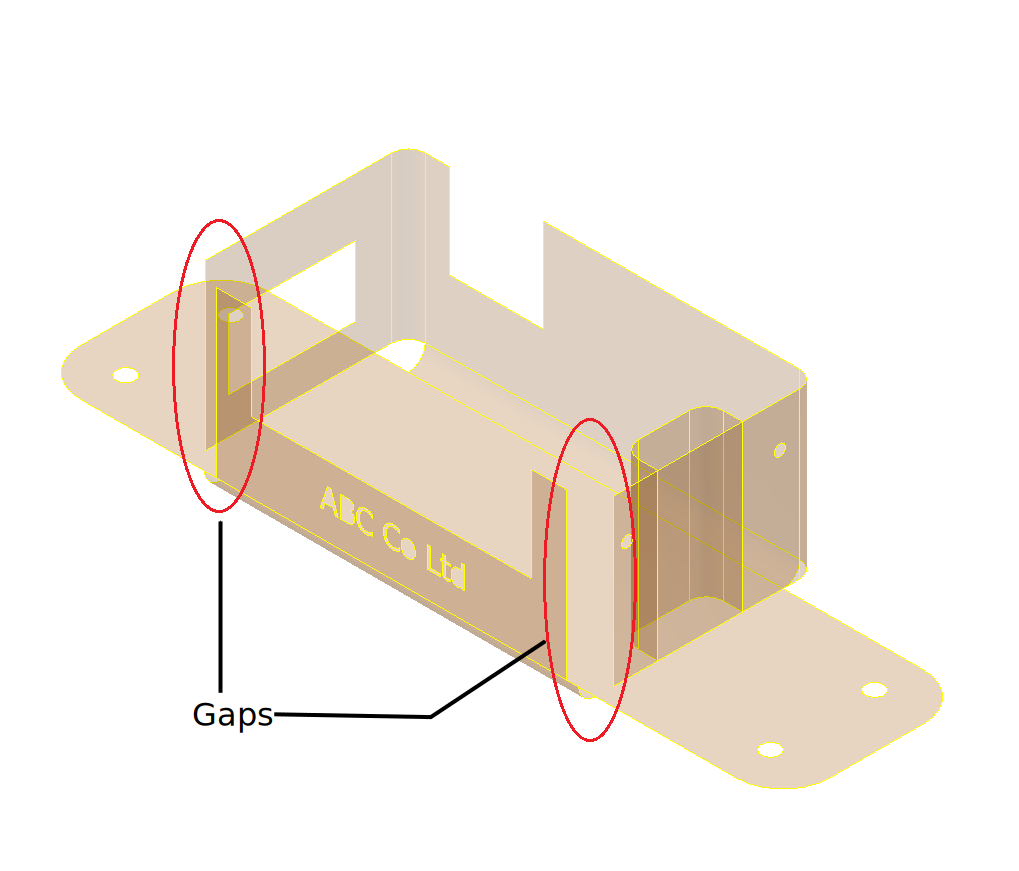
\includegraphics[width=\myfigenlosurebenchmarkcolumnwidth\linewidth,valign=t]{../Common/images/SheetMetal_Medium_Enclosure_InventorMidsurfwithErrors}}
\caption{Computation of Midsurface of an Enclosure Model}
\label{fig:results:enlosurebenchmark}
\end{figure}
%
%\vspace{-0.5cm}

The CAD feature model shows outer casing, two flaps with holes for scree fitments. It has slots for interfaces to external environment. Some superficial features include embossed name and array of slows for guiding wires in place. A chute on one side is to keep the bus-wires in place.
Figure  \ref{fig:results:enlosurebenchmark} shows the ``Enclosure'' part and its midsurface computed by a commercial application. Many failures are observed such as disconnected patches, missing midsurface patches etc. Following sections show progress of the part while going through various modules.

\subsection{Simplification}

Simplification/defeaturing removes unwanted features to compute the ``gross shape''. It also caches tool-bodies of non-suppressible negative features to be used for piercing after midsurface computation. 
Threshold (D) used as a size threshold here is 5\% of the total part size.

\def\myfigenlosuredefeaturecolumnwidth{0.95}
\def\myfigenlosuredefeatureTreecolumnwidth{0.75}

\resizebox{0.7\linewidth}{!}{
\begin{tabular}[h]{@{} p{0.18\linewidth}  p{0.38\linewidth} p{0.1\linewidth} p{0.2\linewidth}@{}}
\toprule
 & Model & Tree & Explanation \\
 \midrule
 
Original/Input &
\raisebox{-0.8\height}{\includegraphics[width=\myfigenlosuredefeaturecolumnwidth\linewidth]{..//Common/images/SheetMetal_Medium_Enclosure_OriginalPart}} &
\raisebox{-0.8\height}{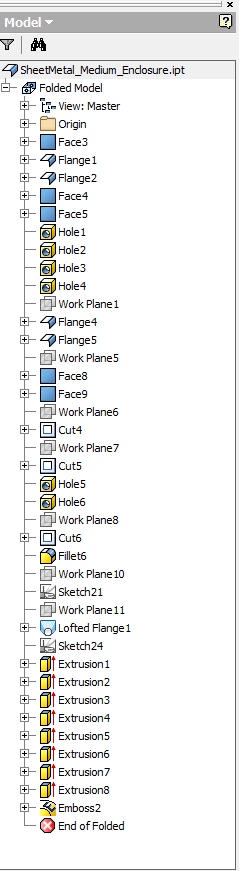
\includegraphics[width=\myfigenlosuredefeatureTreecolumnwidth\linewidth]{..//Common/images/SheetMetal_Medium_Enclosure_OriginalTree}} &

The model has 3 cutouts for components interfacing with outside world, letter-embossing, chute for wires and holes for fixing bolts.\\

Phase I Selections &
\raisebox{-0.8\height}{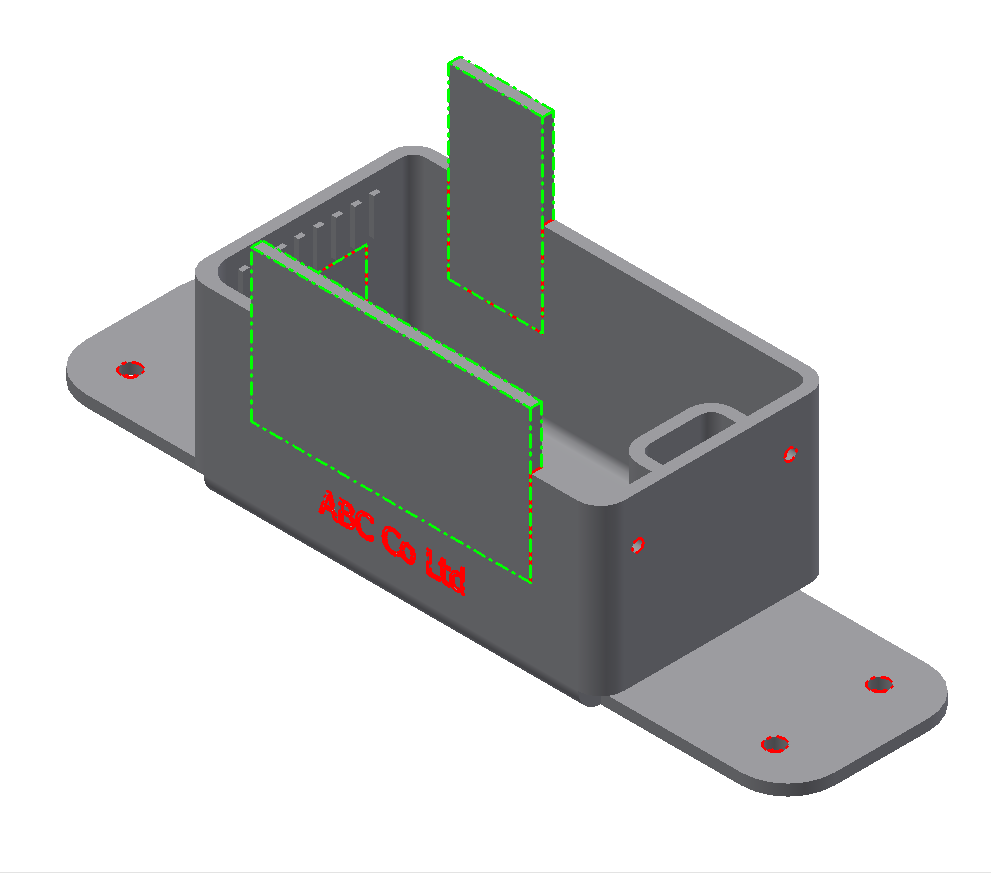
\includegraphics[width=\myfigenlosuredefeaturecolumnwidth\linewidth]{..//Common/images/SheetMetal_Medium_Enclosure_PhaseISelections}} &
\raisebox{-0.8\height}{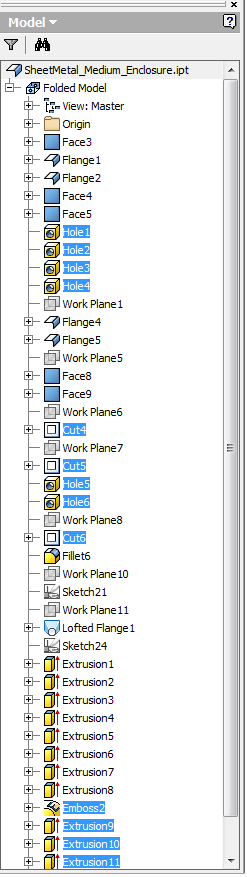
\includegraphics[width=\myfigenlosuredefeatureTreecolumnwidth\linewidth]{..//Common/images/SheetMetal_Medium_Enclosure_PhaseISelectionsTree}} &

Small holes, embossing is chosen based on Sheet Metal feature taxonomy rules (shown in red). The green selections indicate the dormant feature bodies cached.\\

Phase II  Selections&
\raisebox{-0.8\height}{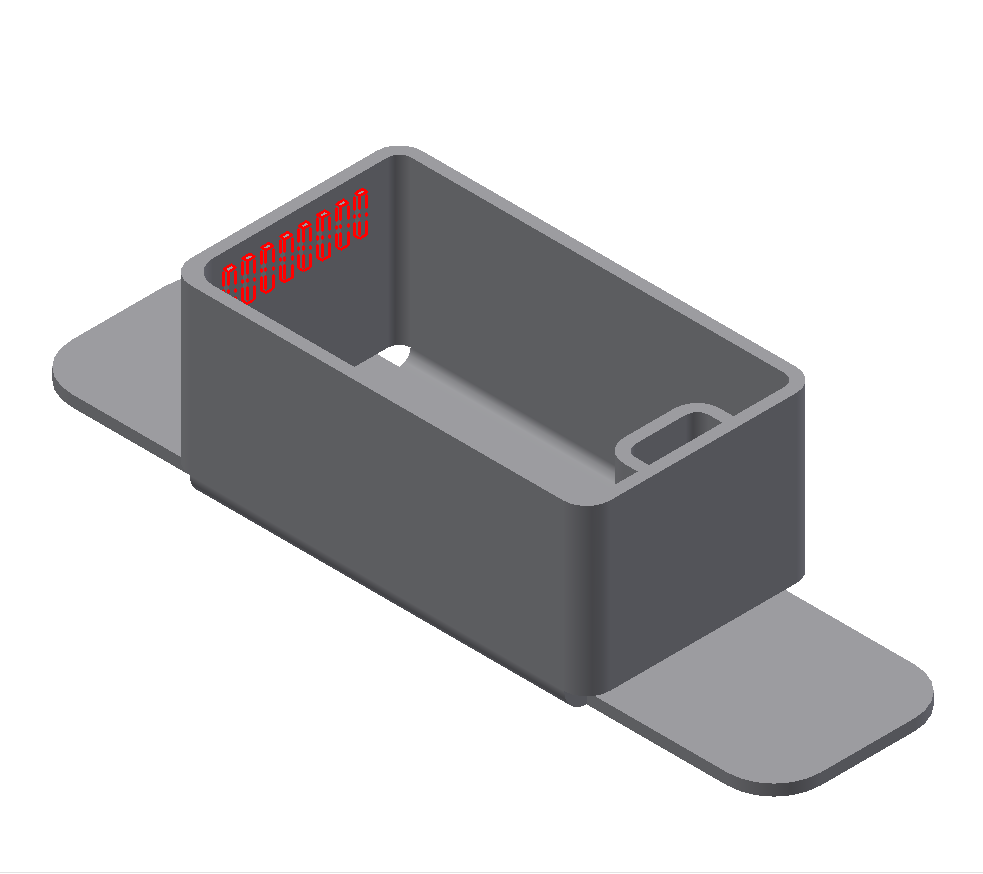
\includegraphics[width=\myfigenlosuredefeaturecolumnwidth\linewidth]{..//Common/images/SheetMetal_Medium_Enclosure_PhaseIISelections}} &
\raisebox{-0.8\height}{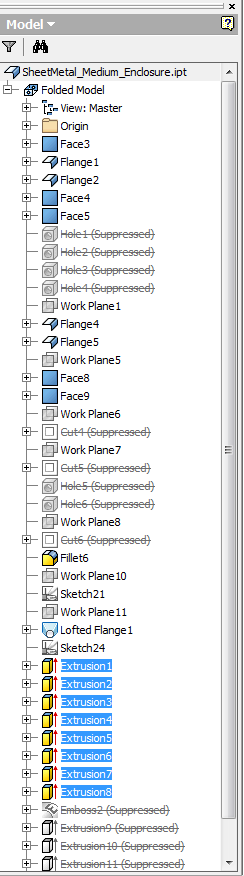
\includegraphics[width=\myfigenlosuredefeatureTreecolumnwidth\linewidth]{..//Common/images/SheetMetal_Medium_Enclosure_PhaseIISelectionsTree}} &

Remnant features get selected in the second phase. \\

Defeatured&
\raisebox{-0.8\height}{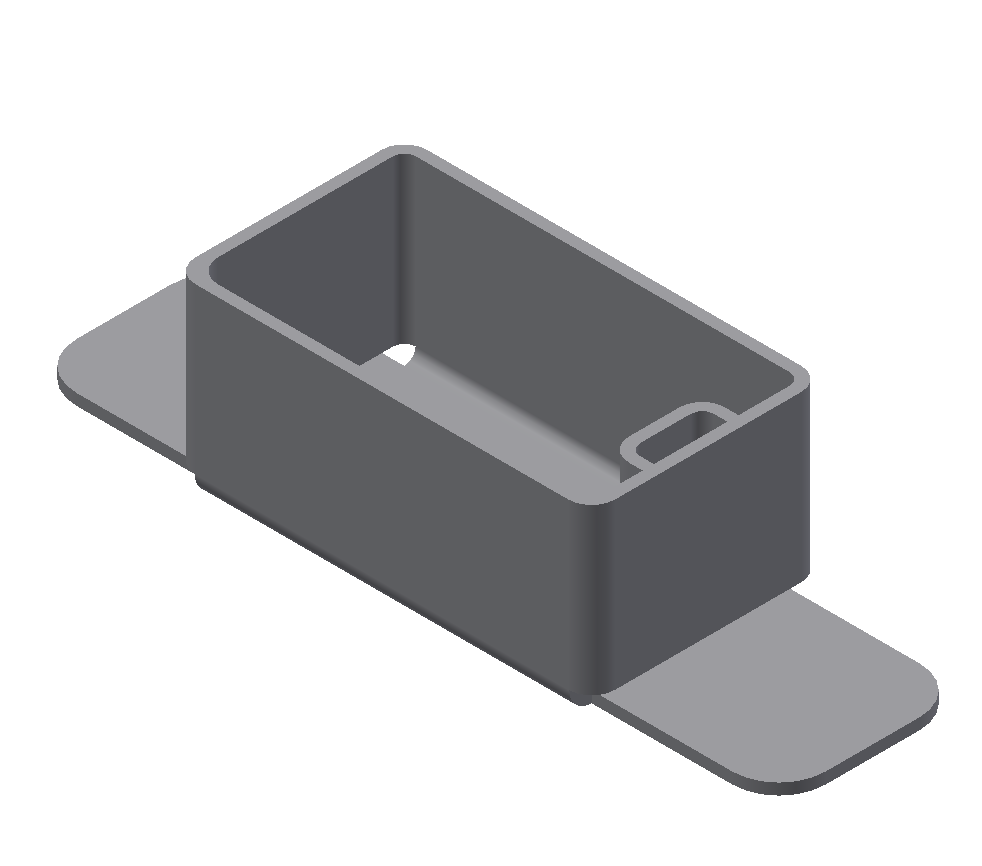
\includegraphics[width=\myfigenlosuredefeaturecolumnwidth\linewidth]{..//Common/images/SheetMetal_Medium_Enclosure_DefeaturedPart}} &
\raisebox{-0.8\height}{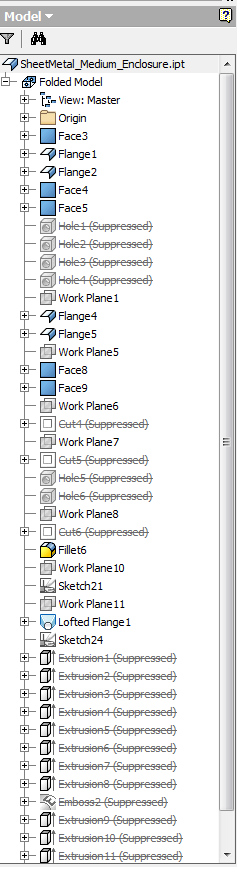
\includegraphics[width=\myfigenlosuredefeatureTreecolumnwidth\linewidth]{..//Common/images/SheetMetal_Medium_Enclosure_DefeaturedTree}} &

Most of the unnecessary features are removed and now it retains all the necessary features adequately ``representing''  the gross shape. \\

\bottomrule
\end{tabular}
}

Effectiveness with 5\% threshold, based on the criterion defined by Eqn. \ref{eqn:defeaturing:effectiveness} is:

\begin{minipage}[c]{0.6\linewidth}
\begin{tabular}[h]{@{} p{0.22\linewidth} p{0.18\linewidth} p{0.21\linewidth} p{0.2\linewidth} @{}}\toprule
\textbf{Qty} & \textbf{Input} & \textbf{Phase I} & \textbf{Output}\\  \midrule
Faces  & 259 & 104 & 64\\
Suppressed  &  &13 & 8\\
\bottomrule
\end{tabular}
\end{minipage}
\begin{minipage}[c]{0.38\linewidth}
$pR = (1 - \frac{64}{259}) \times 100 = 75.29\%$
\end{minipage}

Even after a substantial reduction in the number of faces (75\%), the overall shape of the enclosure is retained fine.

\subsection{Abstraction}

The purpose of this module is to transform sheet metal feature tree into  $\mathcal{ABLE}$ feature (Extrude, Revolve, Sweep, Loft) tree. Effectiveness of this module depends upon the faithful reproduction of the part without any feature or shape loss.

\def\myfigenlosureabelcolumnwidth{0.98}
\resizebox{0.7\linewidth}{!}{
\begin{tabular}[h]{@{} p{0.1\linewidth}  p{0.38\linewidth} p{0.15\linewidth} p{0.2\linewidth}@{}}
\toprule
 & Model & Tree & Explanation \\
 \midrule

Defeatured Input &
\raisebox{-0.8\height}{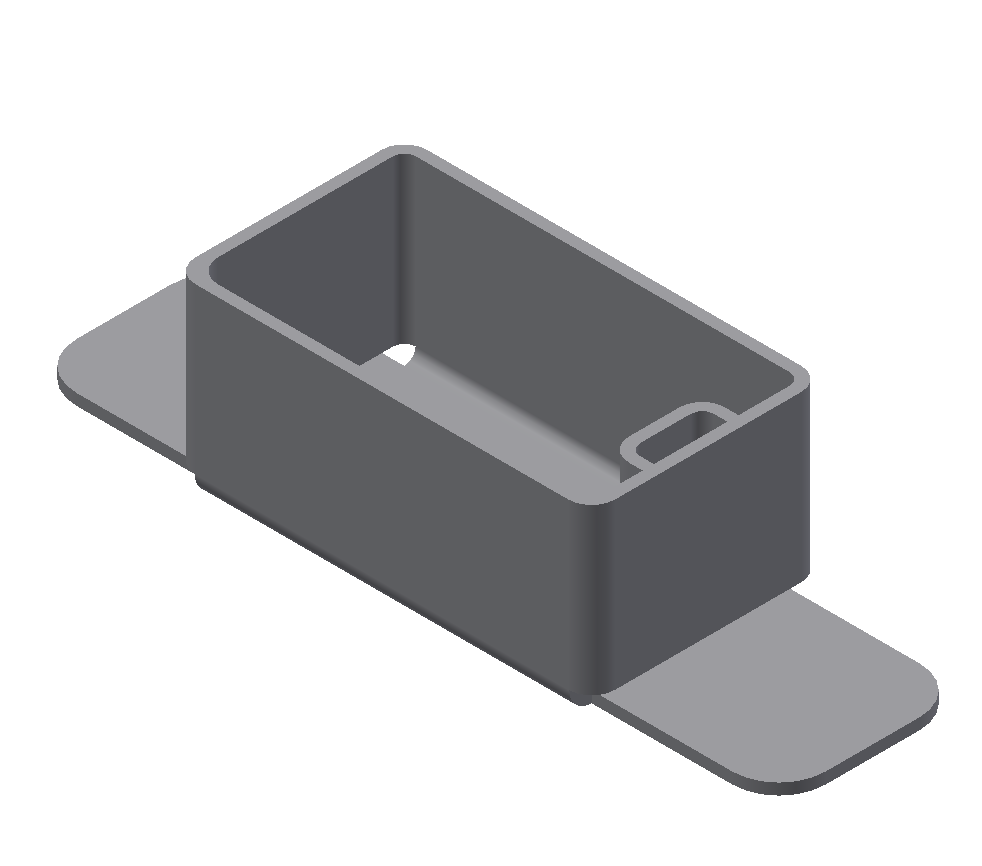
\includegraphics[width=\myfigenlosuredefeaturecolumnwidth\linewidth]{..//Common/images/SheetMetal_Medium_Enclosure_pre_abel_part}} &
\raisebox{-0.8\height}{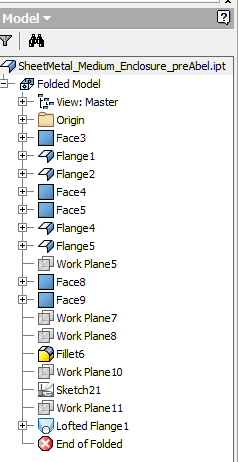
\includegraphics[width=\myfigenlosureabelcolumnwidth\linewidth]{..//Common/images/SheetMetal_Medium_Enclosure_pre_abel_tree}} &

The model has Sheet metal features such as FACE, Flange, Lofted Flange, etc. \\

Abstracted Output &
\raisebox{-0.8\height}{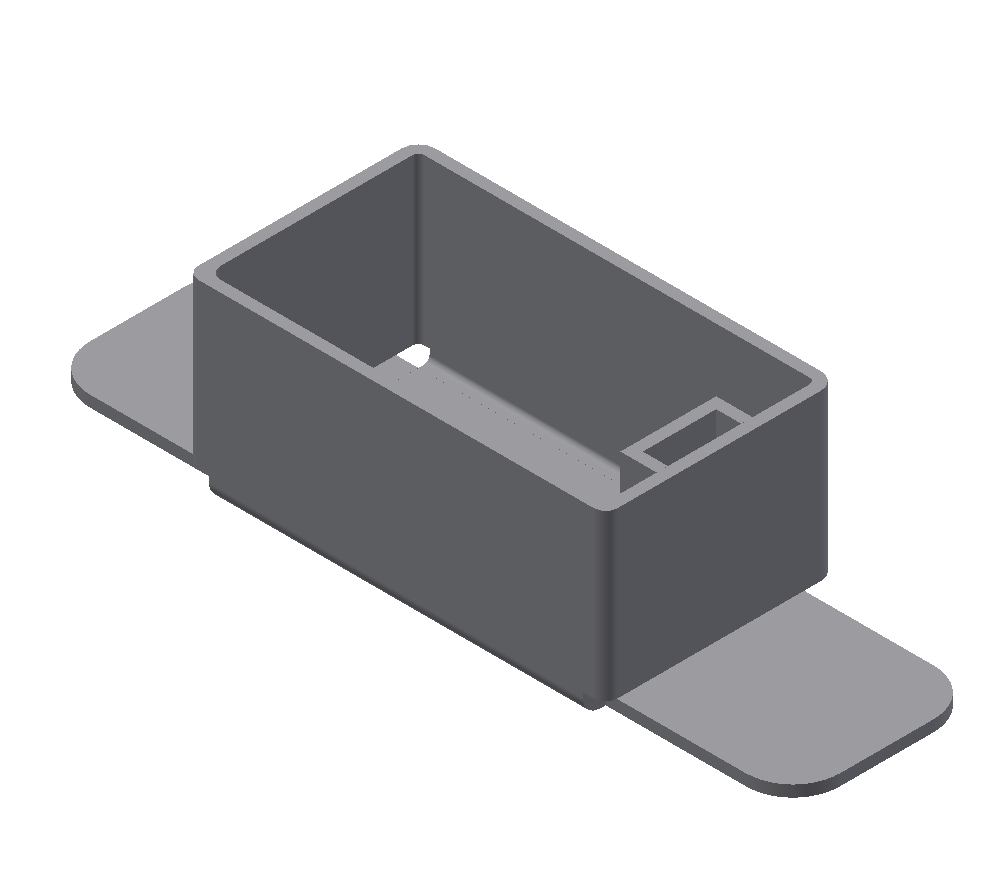
\includegraphics[width=\myfigenlosuredefeaturecolumnwidth\linewidth]{..//Common/images/SheetMetal_Medium_Enclosure_abel_part}} &
\raisebox{-0.8\height}{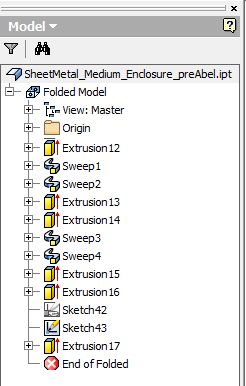
\includegraphics[width=\myfigenlosureabelcolumnwidth\linewidth]{..//Common/images/SheetMetal_Medium_Enclosure_abel_tree}} &

All Sheet Metal features are abstracted/converted to basic primitive features, such as Extrude, Sweep, etc.\\

\bottomrule
\end{tabular}
}
\subsection{Decomposition}

As mentioned in Section \ref{sec:litsurvey:fbcdmidsurf}, many algorithms are readily available and thus are not presented here as they are not contributing to this work. The given abstracted part is decomposed at feature level as well as at convex edges to form sub-volumes/cells.

% The process followed is:
%\begin{itemize}[noitemsep,topsep=2pt,parsep=2pt,partopsep=2pt]
%\item \textbf{Feature partitioning}: Internal as well as external booleans  are changed to the ``New Body'' type, so that the tool-body volumes get separated. The volumes may still overlap with each other.
%\item \textbf{Concave edge partitioning (CEP)}: Overlapping volumes are split at concave edges. Faces at these edges are extended and used as partitions to split. In this work, extensions are not done infinitely (or covering the part's bounding box) but within the influence zone decided by two interacting features.
%\end{itemize}

\def\myfigenlosureabelcolumnwidth{0.98}
\resizebox{0.7\linewidth}{!}{
\begin{tabular}[h]{@{} p{0.1\linewidth}  p{0.38\linewidth} p{0.15\linewidth} p{0.2\linewidth}@{}}
\toprule
 & Model & Tree & Explanation \\
 \midrule

Abstracted Input &
\raisebox{-0.8\height}{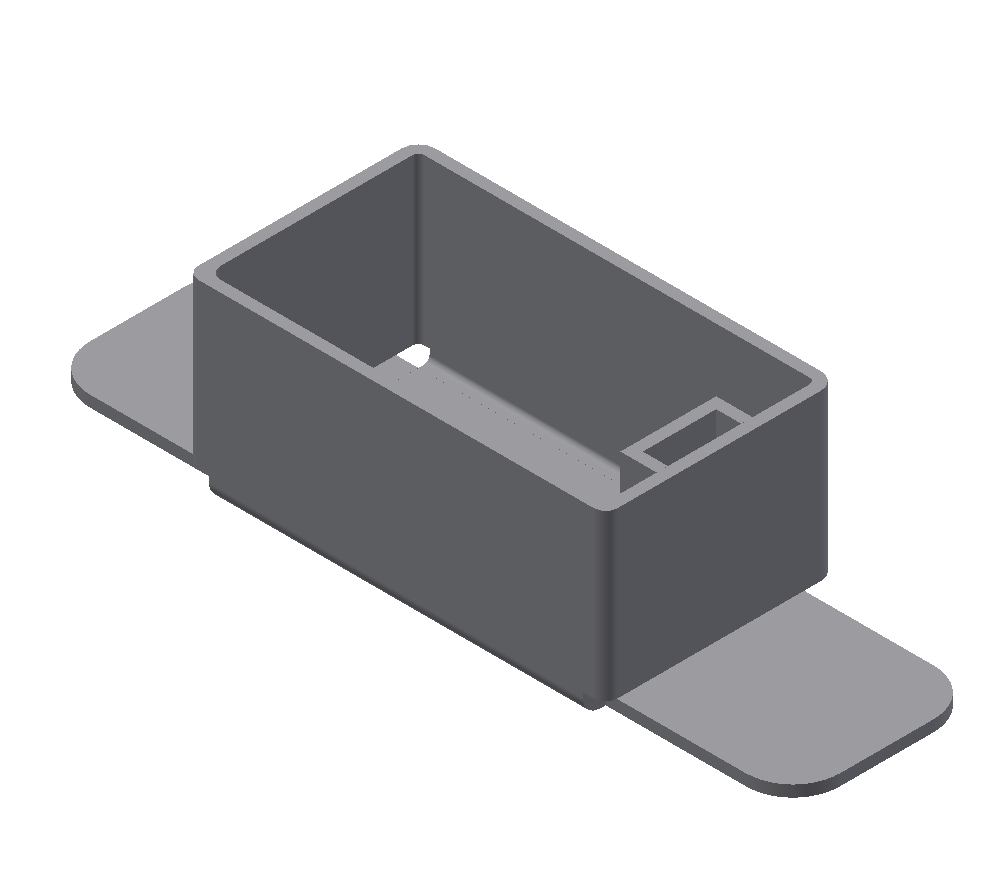
\includegraphics[width=\myfigenlosuredefeaturecolumnwidth\linewidth]{..//Common/images/SheetMetal_Medium_Enclosure_abel_part}} &
\raisebox{-0.8\height}{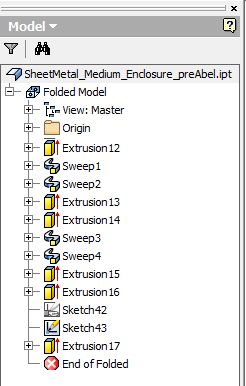
\includegraphics[width=\myfigenlosureabelcolumnwidth\linewidth]{..//Common/images/SheetMetal_Medium_Enclosure_abel_tree}} &

Internal booleans of Primitive features are set to ``New'', thus separating their tool bodies. Later partitioning at convex edges is done.\\

Decomposed Output &
\raisebox{-0.8\height}{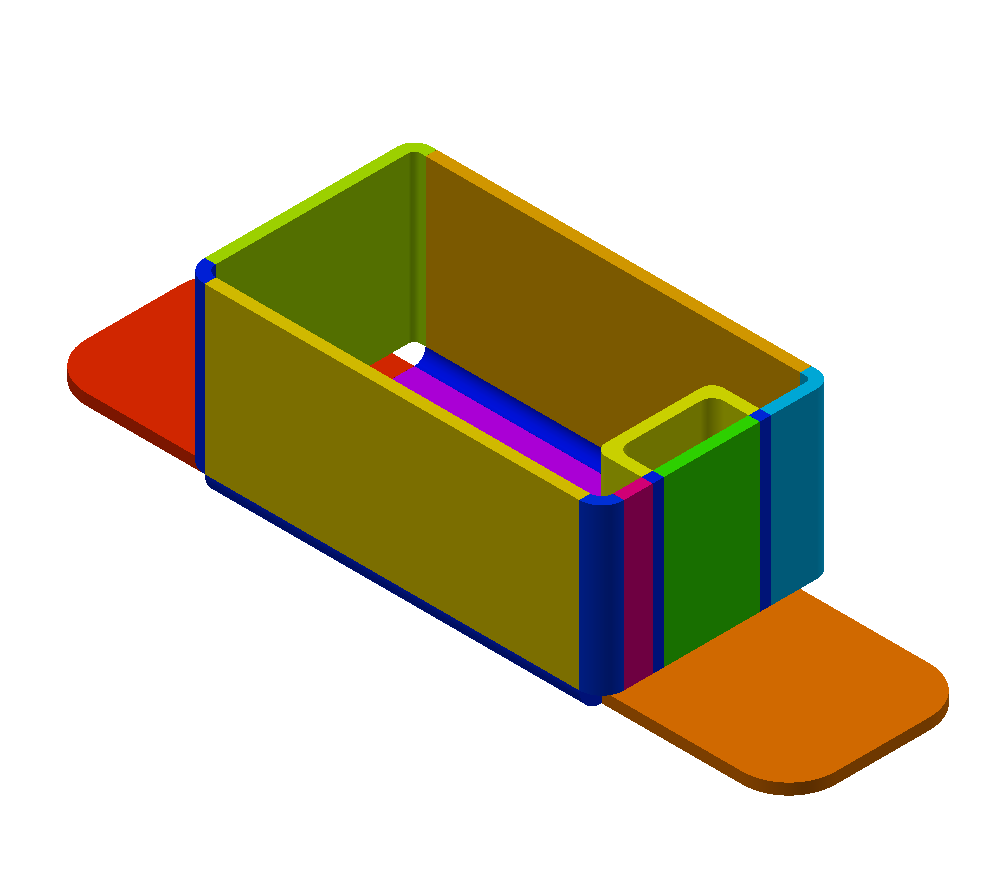
\includegraphics[width=\myfigenlosuredefeaturecolumnwidth\linewidth]{..//Common/images/SheetMetal_Medium_Enclosure_decomp_part}} &
\raisebox{-0.8\height}{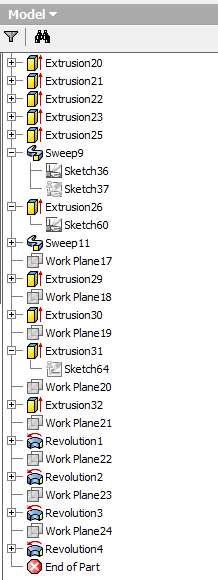
\includegraphics[width=\myfigenlosureabelcolumnwidth\linewidth]{..//Common/images/SheetMetal_Medium_Enclosure_decomp_tree}} &

List of sub-volumes/cells with a primitive/$\mathcal{ABLE}$ owner feature assigned.\\

\bottomrule
\end{tabular}
}
\subsection{Computation}

Midsurface patches and connections are computed to result into a well-connected midsurface of the gross shape. Dormant bodies cached during defeaturing module are brought back to pierce into this midsurface, so as to generate the pending cuts (Figure  \ref{fig:results:dormantenclosure}).

\begin{figure}[!h]
\centering     %%% not \center
\subfloat[Original Part]{\label{fig:results:originalenclosurepart}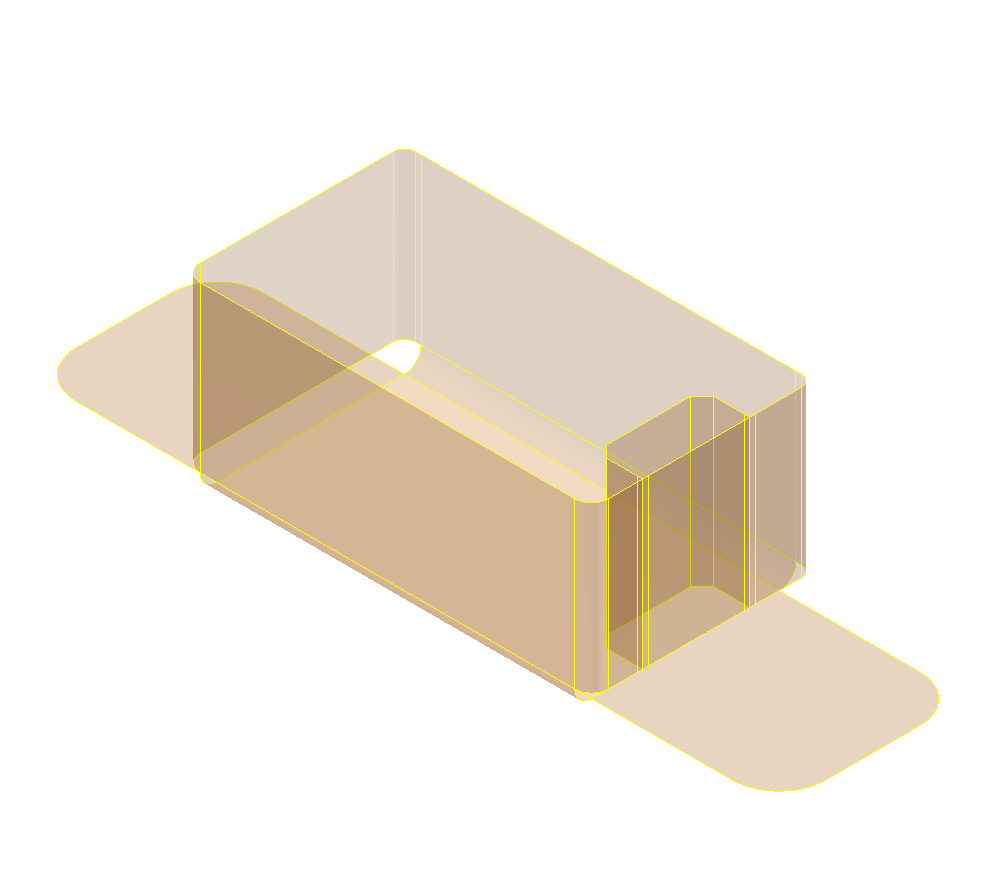
\includegraphics[width=\myfigenlosurebenchmarkcolumnwidth\linewidth,valign=t]{../Common/images/SheetMetal_Medium_Enclosure_midsurf_part}} \qquad
\subfloat[Dormant Piercing]{\label{fig:results:midsurfbyinventorexnclosure}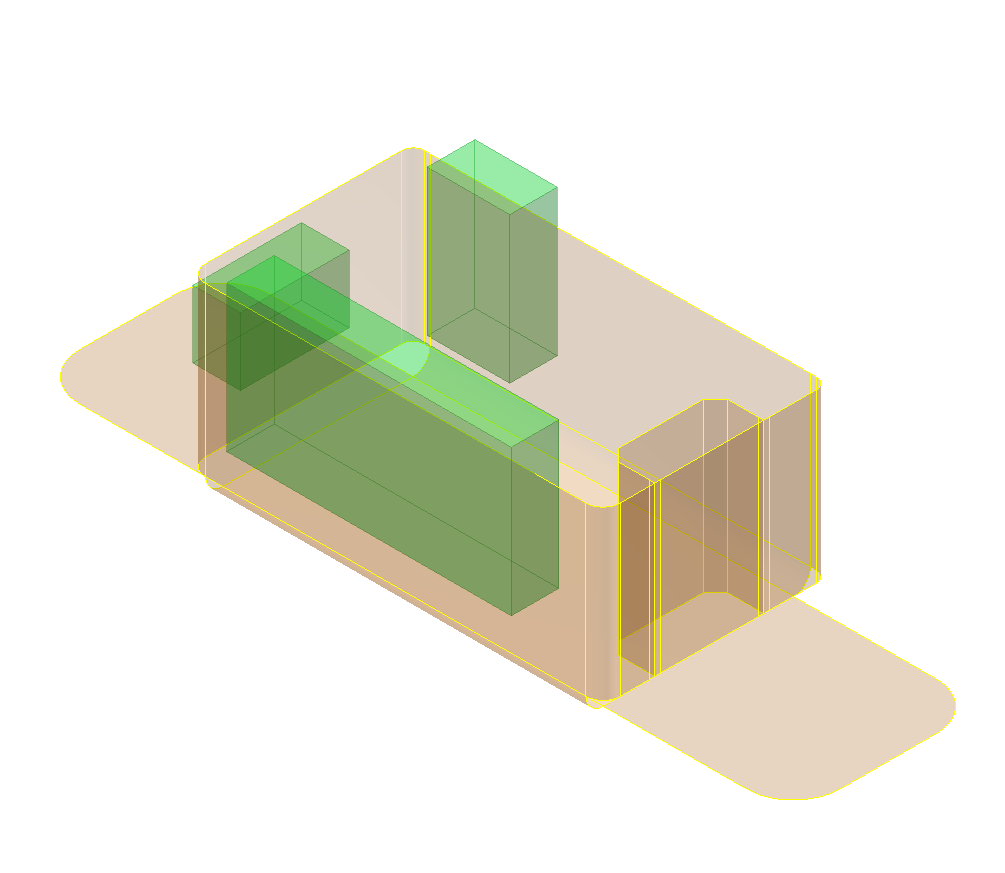
\includegraphics[width=\myfigenlosurebenchmarkcolumnwidth\linewidth,valign=t]{../Common/images/SheetMetal_Medium_Enclosure_dormant_part}}
\caption{Computation of Midsurface and piercing of dormant bodies}
\label{fig:results:dormantenclosure}
\end{figure}

The final midsurface is shown in Figure \ref{fig:results:outputmidsurfenclosure}

\begin{figure}[!htb]
\centering     %%% not \center
\subfloat[Original Part]{\label{fig:results:originalenclosurepart}\includegraphics[width=\myfigenlosurebenchmarkcolumnwidth\linewidth,valign=t]{../Common/images/SheetMetal_Medium_Enclosure_OriginalPart}} \qquad
\subfloat[This Research]{\label{fig:results:mymidsurfenclosure}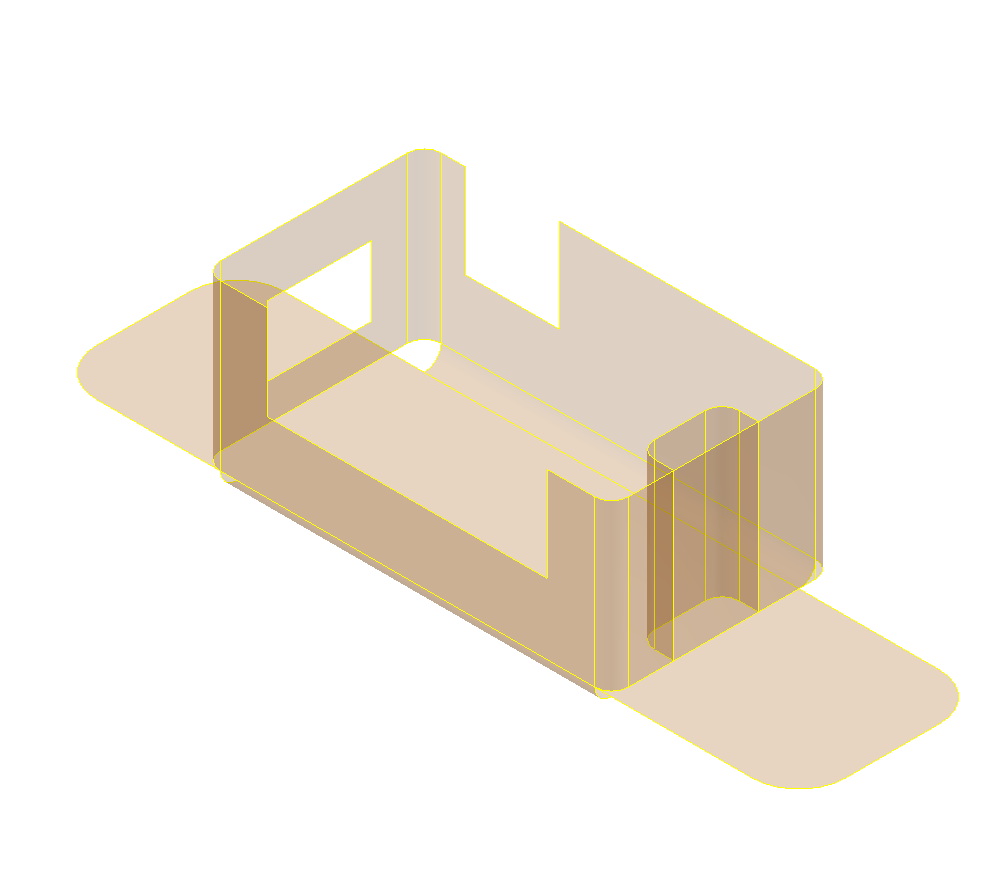
\includegraphics[width=\myfigenlosurebenchmarkcolumnwidth\linewidth,valign=t]{../Common/images/SheetMetal_Medium_Enclosure_final_midsurf_part}}
\caption{Computation of Midsurface of an Enclosure Model}
\label{fig:results:outputmidsurfenclosure}
\end{figure}
